\documentclass[12pt]{article}
\usepackage[danish]{babel}
\usepackage{amsfonts, amssymb, mathtools, amsthm, amsmath}
\usepackage{graphicx, pgfplots}
\usepackage{url}
\usepackage[dvipsnames]{xcolor}
\usepackage{sagetex}
\usepackage{lastpage}

%loaded last
\usepackage[hidelinks]{hyperref}

\usepackage{siunitx}
  \sisetup{exponent-product = \cdot,
    output-decimal-marker = {,}}

%Giles Castelles incfig
\usepackage{import}
\usepackage{xifthen}
\usepackage{pdfpages}
\usepackage{transparent}

\newcommand{\incfig}[2][1]{%
  \def\svgwidth{#1\columnwidth}
  \import{../figures/}{#2.pdf_tex}
}

\setlength{\parindent}{0in}
\setlength{\oddsidemargin}{0in}
\setlength{\textwidth}{6.5in}
\setlength{\textheight}{8.8in}
\setlength{\topmargin}{0in}
\setlength{\headheight}{18pt}

\usepackage{fancyhdr}
\pagestyle{fancy}

\fancyhead{}
\fancyfoot{}
\fancyfoot[R]{\thepage}
\fancyhead[C]{\leftmark}

\pgfplotsset{compat=newest}

\pgfplotsset{every axis/.append style={
  axis x line=middle,    % put the x axis in the middle
  axis y line=middle,    % put the y axis in the middle
  axis line style={<->,color=black}, % arrows on the axis
}}

\usepackage{thmtools}
\usepackage{tcolorbox}
  \tcbuselibrary{skins, breakable}
  \tcbset{
    space to upper=1em,
    space to lower=1em,
  }

\theoremstyle{definition}

\newtcolorbox[auto counter]{definition}[1][]{%
  breakable,
  colframe=ForestGreen,  %frame color
  colback=ForestGreen!5, %background color
  colbacktitle=ForestGreen!25, %background color for title
  coltitle=ForestGreen!70!black,  %title color
  fonttitle=\bfseries\sffamily, %title font
  left=1em,              %space on left side in box,
  enhanced,              %more options
  frame hidden,          %hide frame
  borderline west={2pt}{0pt}{ForestGreen},  %display left line
  title=Definition \thetcbcounter: #1,
}

\newtcolorbox{greenline}{%
  breakable,
  colframe=ForestGreen,  %frame color
  colback=white,          %remove background color
  left=1em,              %space on left side in box
  enhanced,              %more options
  frame hidden,          %hide frame
  borderline west={2pt}{0pt}{ForestGreen},  %display left line
}

\newtcolorbox[auto counter, number within=section]{eks}[1][]{%
  brekable,
  colframe=NavyBlue,  %frame color
  colback=NavyBlue!5, %background color
  colbacktitle=NavyBlue!25,    %background color for title
  coltitle=NavyBlue!70!black,  %title color
  fonttitle=\bfseries\sffamily, %title font
  left=1em,            %space on left side in box,
  enhanced,            %more options
  frame hidden,        %hide frame
  borderline west={2pt}{0pt}{NavyBlue},  %display left line
  title=Eksempel \thetcbcounter: #1
}

\newtcolorbox{blueline}{%
  breakable,
  colframe=NavyBlue,     %frame color
  colback=white,         %remove background
  left=1em,              %space on left side in box,
  enhanced,              %more options
  frame hidden,          %hide frame
  borderline west={2pt}{0pt}{NavyBlue},  %display left line
}

\newtcolorbox{teo}[1][]{%
  breakable,
  colframe=RawSienna,  %frame color
  colback=RawSienna!5, %background color
  colbacktitle=RawSienna!25,    %background color for title
  coltitle=RawSienna!70!black,  %title color
  fonttitle=\bfseries\sffamily, %title font
  left=1em,              %space on left side in box,
  enhanced,              %more options
  frame hidden,          %hide frame
  borderline west={2pt}{0pt}{RawSienna},  %display left line
  title=Teori: #1,
}

\newtcolorbox[auto counter, number within=section]{sæt}[1][]{%
  breakable,
  colframe=RawSienna,  %frame color
  colback=RawSienna!5, %background color
  colbacktitle=RawSienna!25,    %background color for title
  coltitle=RawSienna!70!black,  %title color
  fonttitle=\bfseries\sffamily, %title font
  left=1em,              %space on left side in box,
  enhanced,              %more options
  frame hidden,          %hide frame
  borderline west={2pt}{0pt}{RawSienna},  %display left line
  title=Sætning \thetcbcounter: #1,
  before lower={\textbf{Bevis:}\par\vspace{0.5em}},
  colbacklower=RawSienna!25,
}

\newtcolorbox{redline}{%
  breakable,
  colframe=RawSienna,  %frame color
  colback=white,       %Remove background color
  left=1em,            %space on left side in box,
  enhanced,            %more options
  frame hidden,        %hide frame
  borderline west={2pt}{0pt}{RawSienna},  %display left line
}

\newtcolorbox{for}[1][]{%
  breakable,
  colframe=NavyBlue,  %frame color
  colback=NavyBlue!5, %background color
  colbacktitle=NavyBlue!25,    %background color for title
  coltitle=NavyBlue!70!black,  %title color
  fonttitle=\bfseries\sffamily, %title font
  left=1em,              %space on left side in box,
  enhanced,              %more options
  frame hidden,          %hide frame
  borderline west={2pt}{0pt}{NavyBlue},  %display left line
  title=Forklaring #1,
}

\newtcolorbox{bem}{%
  breakable,
  colframe=NavyBlue,  %frame color
  colback=NavyBlue!5, %background color
  colbacktitle=NavyBlue!25,    %background color for title
  coltitle=NavyBlue!70!black,  %title color
  fonttitle=\bfseries\sffamily, %title font
  left=1em,              %space on left side in box,
  enhanced,              %more options
  frame hidden,          %hide frame
  borderline west={2pt}{0pt}{NavyBlue},  %display left line
  title=Bemærkning:,
}

\makeatother
\def\@lecture{}%
\newcommand{\lecture}[3]{
  \ifthenelse{\isempty{#3}}{%
    \def\@lecture{Lecture #1}%
  }{%
    \def\@lecture{Lecture #1: #3}%
  }%
  \subsection*{\makebox[\textwidth][l]{\@lecture \hfill \normalfont\small\textsf{#2}}}
}

\makeatletter

\newcommand{\opgave}[1]{%
 \def\@opgave{#1}%
 \subsection*{Opgave #1}
}

\makeatother

%Format lim the same way in intext and in display
\let\svlim\lim\def\lim{\svlim\limits}

% horizontal rule
\newcommand\hr{
\noindent\rule[0.5ex]{\linewidth}{0.5pt}
}

\title{Eksamen i: Fysik og Mekanik}
\author{Noah Rahbek Bigum Hansen}
\date{21. december 2022 (14. December 2024)}

\begin{document}

\maketitle

\section*{1.}
\begin{figure} [ht]
  \centering
  \caption{}
  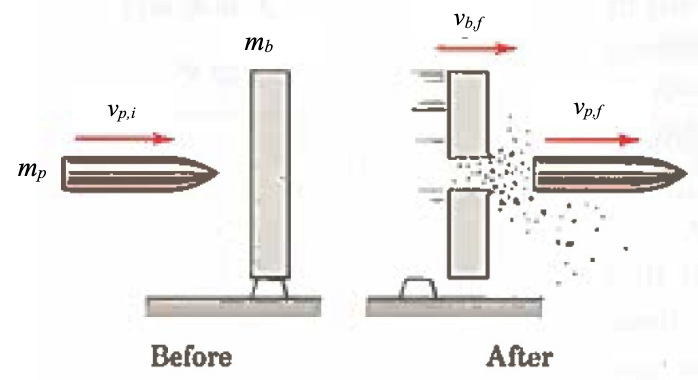
\includegraphics[width=0.5\linewidth]{../figures/E3_1.png}
  \label{fig:E3_1}
\end{figure}

Et projektil med massen $m_p$ affyres vandret med farten $v_{p,i}$ ind i en stationær træblok med massen $m_b$ .  Projektilet passerer gennem træblokken og kommer ud gennem ``bagsiden'' med farten $v_{p,f}$. Bestem træblokkens endelige fart $v_{b,f}$, udtrykt ved de øvrige givne størrelser ($m_p, m_b, v_{p,i}, v_{p,f}$). Friktionen mellem træblokken og understøtningen/bordet (se \textbf{\autoref{fig:E3_1}}) kan antages at være forsvindende lille.
\bigbreak
Fra impulsbevarelse har vi at
\[ 
m_p \cdot v_{p,i} = m_p \cdot v_{p,f} + m_b \cdot v_{b,f}
.\]
Heri kan træblokkens fart efter sammenstødet isoleres som
\begin{align*}
  v_{b,f} &= \frac{m_p \cdot v_{p,i} - m_p \cdot v_{p,f}}{m_b} \\
  v_{b,f} &= \frac{m_p \left( v_{p,i} - v_{p,f} \right)}{m_b}
.\end{align*}
Altså er træblokkens fart efter sammenstødet $v_{b,f} = \frac{m_p \left( v_{p,i} - v_{p,f} \right)}{m_b}$


\section*{2.}
\begin{figure} [ht]
  \centering
  \caption{}
  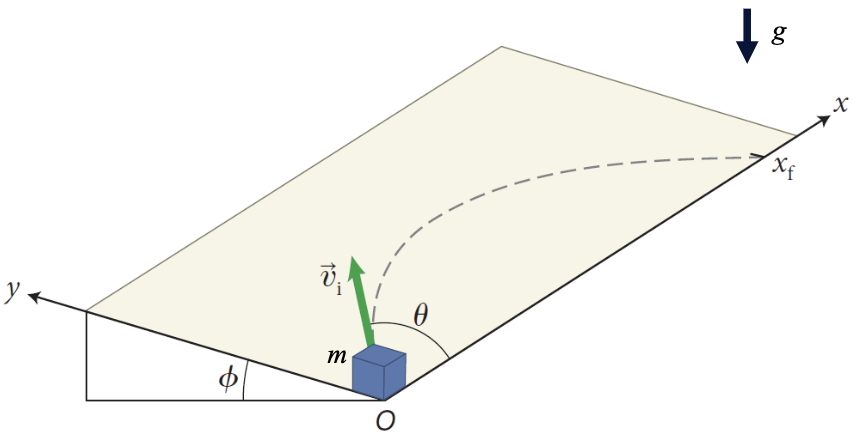
\includegraphics[width=0.5\linewidth]{../figures/E3_2.png}
  \label{fig:E3_2}
\end{figure}

Massen $m$ er, for tider $t < 0$, i hvile i origo af et $xy$-koordinatsystem forbundet til et skråplan som har en hældning $\phi$ i forhold til vandret (\textbf{\autoref{fig:E3_2}}). Til tiden $t = 0$ ``affyres'' massen $m$ nu op ad skråplanet med starthastigheden $\Vec{v}_i$. Vinklen mellem $\Vec{v}_i$ og $x$-aksen er givet ved $\theta$, se igen \textbf{\autoref{fig:E3_2}}. Tyngdeaccelerationen betegnes med $g$. Friktion kan ignoreres.


\subsection*{(a)}
Hvad er størrelsen og retningen af blokkens acceleration $\Vec{a}$ i det angivne koordinatsystem? (Udtryk $\Vec{a}$ ved enhedsvektorerne $\hat{\imath}$ og $\hat{\jmath}$, dvs. på formen $\Vec{a} = a_x \hat{\imath} + a_y \hat{\jmath}$.)
\bigbreak
\begin{figure}[ht]
  \centering
  \incfig[0.5]{E31}
  \caption{Fritlegemediagram}
  \label{fig:E31}
\end{figure}

Tyngdekraft-komposanten der peger `nedad' i det angivne koordinatsystem $\overline{F}_g$ kan findes som
\[ 
\overline{F}_g = \sin \phi \cdot F_g = \sin \phi mg
.\]
Massens acceleration kan da findes vha. Newtons 2. lov idet den eneste kraft der virker på massen er tyngdekraften. Dette gøres som så
\begin{align*}
  F &= ma \\
  \implies a &= \frac{F}{m} \\
  \implies a_b &= \frac{\overline{F}_g}{m} = \frac{\sin \phi mg}{m} = \sin\phi g
.\end{align*}
Tyngdekraften virker kun i retningen $-y$ således er $\Vec{a}$ givet ved
\[ 
\Vec{a} = a_x \hat{\imath} + a_y \hat{\jmath} = - \sin \phi \cdot  g \, \hat{\jmath}
.\]


\subsection*{(b)}
Udled et udtryk for massens hastighed som funktion af tiden $t$ ($t > 0$), ligeledes udtrykt i enhedsvektorerne for det angivne koordinatsystem.
\bigbreak
Massens hastighed til en given tid $t$ kan findes vha. formlen for hastighed ved konstant acceleration som ser ud som følger
\[ 
v = v_{0} + at
.\]
I $x$-retningen er der ingen kraft og dermed ingen acceleration og derfor er hastigheden i denne retning konstant
\[ 
v_x = \cos \theta \cdot v_i
.\]
I $y$-retningen virker der en kraft på massen og den får dermed en acceleration. Kraften der virker på massen er tyngdekraften, og denne er derfor konstant, hvilket medfører en konstant acceleration. Denne er fundet ovenfor til $a_y = - \sin \phi \cdot g$. Dermed fås altså
\[ 
v_y = \sin \theta \cdot v_i - \sin \phi \cdot g \cdot t
.\]
Altså bliver det samlede udtryk for $\Vec{v}(t)$
\[ 
\Vec{v}(t) = v_x \hat{\imath} + v_y \hat{\jmath} = \left( \cos \theta \cdot v_i \right) \hat{\imath} + \left( \sin \theta \cdot v_i - \sin\phi \cdot g t \right) \hat{\jmath}
.\]




\subsection*{(c)}
Hvad er den maksimale værdi af forskydning $\Delta y$ langs $y$-aksen?
\bigbreak
Idet origo sættes til det punkt hvor massen starter tilsvarer den maksimale værdi af forskydning langs $y$-aksen, $\Delta y$, den maksimale højde i kastet. For at finde ud af hvornår højden er maksimeret findes tiden $t$ til $v_y = 0$. Altså har vi at
\begin{align*}
  v_y &= 0 \\
  0 &= \sin \theta \cdot v_i - \sin \phi \cdot gt \\
  \sin \phi \cdot gt &= \sin\theta \cdot v_i\\
  t &= \frac{\sin \theta \cdot v_i}{\sin \phi \cdot g}
.\end{align*}
Denne værdi for $t$, hvor hastigheden er $0$ kan nu indsættes i formlen for højden ved et skråt kast, som generelt ser ud som
\[ 
y = (v_i \cdot \sin \theta)t - \frac{1}{2}at^2
.\]
Sættes udtrykket for tiden $t$ ind fås at
\begin{align*}
  y_{maks} &= \left( v_i \cdot \sin\theta \right) \cdot \frac{\sin\theta \cdot v_i}{\sin \phi \cdot g} - \frac{1}{2} \cdot \left( -\sin\phi \cdot g \right) \cdot \left( \frac{\sin \theta \cdot v_i}{\sin \phi \cdot g} \right)^2\\
  &= \frac{\sin^2 \theta \cdot v_i^2}{\sin \phi \cdot g} - \frac{1}{2} \cdot \frac{\sin^2 \theta \cdot v_i^2}{\sin \phi \cdot g} \\
  &= \frac{1}{2} \cdot \frac{\sin^2 \theta \cdot v_i^2}{\sin\phi \cdot g}
.\end{align*}



\subsection*{(d)}
Hvad er blokkens maksimale forskydning $\Delta x$ langs $x$-aksen?
\bigbreak
Den maksimale forskydning $\Delta x$ langs $x$-aksen, forstås i dette tilfælde som den maksimale afstand som blokken kommer til at bevæge sig før den glider ned af pladen (det punkt, der er betegnet $x_{f}$ på fritlegemediagrammet). Altså skal findes det tidspunkt $t$ hvor højden $y = 0$. Vi får altså
\[ 
y = 0 \implies (v_i \cdot \sin \theta)t - \frac{1}{2}at^2 = 0
.\]
Denne omskrives som
\begin{align*}
  v_i \cdot \sin\theta \cdot t &= \frac{1}{2}at^2 \\
  v_i \cdot \sin\theta &= \frac{1}{2}at \\
  t &= \frac{2\cdot v_i \cdot \sin\theta}{a}
.\end{align*}
Bemærk, at vi grundet division med $t$ forkaster den løsning, hvor $t = 0$, dette er dog ikke et problem da dette er starttidspunktet og blokken ikke vil falde af blokken med det samme, medmindre enten $v_i = 0$ eller $\sin\theta = 0$, hvilket ikke vil give mening ift. opgaven. Dette udtryk for $t$ kan nu indsættes i formlen for horisontal afstand i et skråt kast som ser ud som følger
\[ 
x = v_0 \cdot \cos \theta \cdot t \implies x = v_i \cdot \cos\theta \cdot \frac{2 \cdot v_i \cdot \sin\theta}{g\cdot \sin\phi}
.\]
Dette omskrives til
\[
  \Delta x_{max} = \frac{2 \cdot v_i^2 \cos \theta \cdot \sin\theta}{g\cdot \sin\phi}
.\]


\section*{3.}
\begin{figure} [ht]
  \centering
  \caption{}
  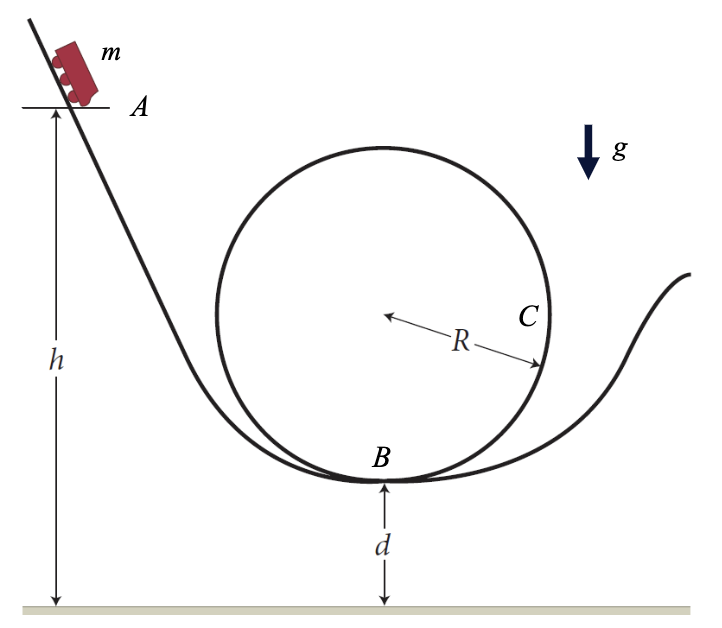
\includegraphics[width=0.5\linewidth]{../figures/E3_3.png}
  \label{fig:E3_3}
\end{figure}

En rutsjebanevogn med massen $m$, hvis begyndelsesposition (position $A$) er i højden $h$ over jorden, begynder en nedadgående tur langs et langt, stejlt skrånende sæt skinner, for derefter at gå ind i et cirkulært loop (”loop-the loop”) med radius $R$, hvis bund er i afstanden $d$ over jorden (\textbf{\autoref{fig:E3_3}}). Tyngdeaccelerationen betegnes med $g$. Friktion kan ignoreres.

\subsection*{(a)}
Hvad er vognens hastighed når den når bunden af loopet (position $B$)?
\bigbreak
Idet friktionen kan ignoreres er der mekanisk energibevarelse. Vi har altså at
\[ 
k_{0} + U_{0} = k_{1} + U_{1}
.\]
Derudover er $k_0 = 0$ idet vognen ikke har en hastighed i starten og $U_1 = 0$ da højdens nulpunkt sættes til højden til punktet $B$. Vi får altså at
\[ 
mg(h-d) = \frac{1}{2}mv_B^2 
.\]
Heri kan hastigheden til punktet $B$ isoleres som
\begin{align*}
  \frac{1}{2}v_B^2 = g(h-d) \\
  v_B = \sqrt{2g(h-d)}
.\end{align*}
Altså er vognens hastighed til punktet $B$ \underline{\underline{$v_B = \sqrt{2g(h-d)}$}}.

\subsection*{(b)}
Hvad er størrelsen af normalkraften virkende på vognen i det øjeblik?
\bigbreak
De eneste to kræfter der virker på vognen i bunden af loopet udover normalkraften er centripetalkraften og tyngdekraften. Vi har altså at
\[ 
N_B = F_{t,b} + F_{cen}
.\]
Centripetalkraften er givet som
\[ 
F_{cp} = m a_r = m \cdot \frac{v^2_{tan}}{R} = m\frac{v_B^2}{R}
.\]
Og tyngdekraften kan findes med Newtons 2. lov som
\[ 
F_{t,b} = mg
.\]
Normalkraften $N_B$ må da være
\[ 
N_B = m \left( g + \frac{v_B^2}{R} \right)
.\]
Sættes udtrykker for $v_B$ fundet i sidste opgave ind fås at normalkraften er
\begin{align*}
  N_B &= m \left( g + \frac{2g(h-d)}{R} \right) \\
  &= mg \left( 1 + 2 \cdot \frac{h-d}{R} \right)
.\end{align*}



\subsection*{(c)}
Hvad er vognens hastighed, når dens position er en fjerdedel af vejen rundt om loopet (position $C$)?
\bigbreak
I dette tilfælde har vi igen en mekanisk energibevarelse og dermed at
\[ 
k_{B} + U_{B} = k_{C} + U_{C} \implies \frac{1}{2}mv_B^2 + 0 = \frac{1}{2}mv_C^2 + mgR
.\]
Heri kan vognens hastighed ved punkt $C$, $v_C$ isoleres som
\begin{align*}
  \frac{1}{2}mv_C^2 &= \frac{1}{2}mv_B^2 - mgR \\
  v_C &= \sqrt{v_B^2 - 2gR} \\
  v_C &= \sqrt{2g(h-d) - 2gR} \\
  v_C &= \sqrt{2g(h-d-R)}
.\end{align*}

\subsection*{(d)}
Hvad er størrelsen af normalkraften på vognen i position $C$?
\bigbreak
Til punktet $C$ kommer tyngdekraften ikke til at bidrage til normalkraften, da tyngdekraften er parallel med skinneren netop i dette punkt. Derfor må hele bidraget komme fra centripetalkraften. Vi har dermed at
\[ 
N_C = m \frac{v_C^2}{R} = m \cdot \frac{2g(h-d-R)}{R}
.\]



\subsection*{(e)}
Hvad er vognens acceleration i position $C$?
\bigbreak
De kræfter der virker på vognen i position $C$ er tyngdekraften (nedad) og centripetalkraften (indad). Vi har tidligere fundet udtryk for disse to som
\begin{align*}
  F_{g,C} &= mg \\
  F_{cp} &= m \frac{v_C^2}{R} = m \frac{2g(h-d-R)}{R}
.\end{align*}
For at omregne disse to til accelerationer kan vi blot dividere med massen $m$ jf. Newtons 2. lov som
\begin{align*}
  a_{g,C} &= g \\
  a_{cp} &= 2g\frac{h-d-R}{R}
.\end{align*}
Den samlede acceleration er vektorsummen af disse to. Tegnes et almindeligt koordinatsystem således at både tyngdekraften og centripetalkraften virker i negativ retning bliver accelationsvektoren altså
\[ 
\Vec{a} = -g \hat{\imath} - 2g \frac{h-d-R}{R} \hat{\jmath} = -g \left( \hat{\imath} + 2 \frac{h-d-R}{R} \hat{\jmath} \right)
.\]



\section*{4.}
\begin{figure} [ht]
  \centering
  \caption{}
  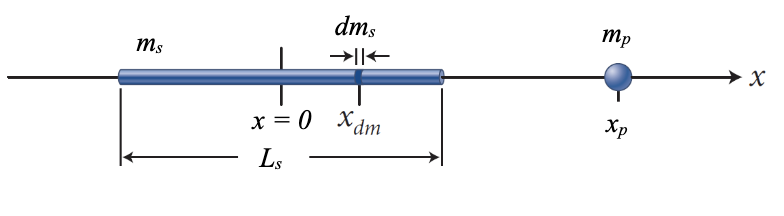
\includegraphics[width=0.5\linewidth]{../figures/E3_4.png}
  \label{fig:E3_4}
\end{figure}

En jævntyk stang med massen $m_s$ og længden $L_s$ er placeret langs aksen $x$, langt fra nogen stjerne eller planet, med stangens midtpunkt i $x = 0$ (\textbf{\autoref{fig:E3_4}}). En punktmasse $m_p$ er placeret i $x = x_p$.

\subsection*{(a)}
Opskriv et udtryk for den til massetiltrækningen hørende potentielle energi $U$ for et system bestående af punktmassen $m_p$ og et lille infinitesimalt element $\mathrm{d}m_s$ af stangen, placeret i $x = x_{dm}$ ($x_{dm} > 0$). Vink: Vi kan skrive $\mathrm{d}m_s = \frac{m_s}{L_s} \, \mathrm{d}x_{dm}$, hvor $\mathrm{d}x_{dm}$ er længden af elementet $\mathrm{d}m_s$.
\bigbreak
Vi har fra opgaven at
\[ 
  \mathrm{d}m_s = \frac{m_s}{L_s}\mathrm{d}x_{dm}
.\]
Den potentielle energi i et tyngdefelt er generelt givet som
\[ 
U = - G \frac{Mm}{r}
.\]
Afstanden $r$ mellem de to masser er $x_p - x_{dm}$, de to masser er $m = m_p$ og $M = \mathrm{d}m_s$. Vi får derfor flg. udtryk for den infinitesimale potentielle energi mellem den infinitesimale del af stangen og punktmassen
\[ 
\mathrm{d}U = -G \frac{\mathrm{d}m_s \cdot m_p}{x_p - x_{dm}} = - G \frac{m_s \cdot m_p \, \mathrm{d}x_{dm}}{L_s(x_p - x_{dm})}
.\]

\subsection*{(b)}
Integrer det i spørgsmål (a) fundne udtryk over stangens længde, og bestem således systemets potentielle energi for $x_p > \frac{L_s}{2}$.
\bigbreak
Vi opstiller først integralet som
\[ 
U = \int_{-\frac{L_s}{2}}^{\frac{L_s}{2}} -\frac{G \cdot m_s \cdot m_p}{L_s} \frac{\mathrm{d}x_{dm}}{x_p - x_{dm}} = -\frac{G \cdot m_s \cdot m_p}{L_s} \int_{- \frac{L_s}{2}}^{\frac{L_s}{2}} \frac{\mathrm{d}x_{dm}}{x_p - x_{dm}}
.\]
Vi sætter $k = \frac{G \cdot m_s \cdot m_p}{L_s}$ i det følgende for at lette opskrivningen. Vi sætter $g(x_{dm}) = x_p - x_{dm}$ og kan derfor benytte kædereglen på $\mathrm{d}x_{dm}$ som
\begin{align*}
  U &= -k \int_{-\frac{L_s}{2}}^{\frac{L_s}{2}} \frac{- \mathrm{d}(x_p - x_{dm})}{x_p - x_{dm}} \\
  &= k \int_{- \frac{L_s}{2}}^{\frac{L_s}{2}} \frac{1}{x_p - x_{dm}} \, \mathrm{d}(x_p - x_{dm}) \\
  &= k \left[ \ln(x_p - x_{dm}) \right]_{- \frac{L_s}{2}}^{\frac{L_s}{2}} \\
  &= k \left( \ln (x_p - \frac{L_s}{2}) - \ln(x_p + \frac{L_s}{2}) \right) \\
  &= k \ln \left( \frac{x_p - \frac{L_s}{2}}{x_p + \frac{L_s}{2}} \right) \\
  &= \frac{G m_s m_p}{L_s} \ln \left( \frac{x_p - \frac{L_s}{2}}{x_p + \frac{L_s}{2}} \right)
.\end{align*}


\subsection*{(c)}
Det kan vises, at for et system som det her givne, er massetiltrækningskraften mellem stangen og punktmassen givet ved $F_x = - \frac{\mathrm{d}U}{\mathrm{d}x}$. Udregn (evaluer) kraften $F_x$ for det givne system, med punktmassen placeret i et vilkårligt $x = x_p$ (dog stadig med $x_p > \frac{L_s}{2}$).
\bigbreak
Vi kan indsætte udtrykket fundet i sidste opgave i formlen fra opgaven som
\[
  - F_x = \frac{\mathrm{d}}{\mathrm{d}x_p} k \ln \left( \frac{x_p - \frac{L_s}{2}}{x_p + \frac{L_s}{2}} \right)
.\]
Vi sætter $f(x_p) = \frac{x_p - \frac{L_s}{2}}{x_p + \frac{L_s}{2}}$ og får dermed et udtryk på formen $\frac{\mathrm{d}}{\mathrm{d}x} \ln(f(x)) = \frac{1}{f_x} \frac{\mathrm{d}f(x)}{\mathrm{d}x}$. Vi får dermed at
\begin{align*}
  -F_x &= k \cdot \frac{x_p + \frac{L_s}{2}}{x_p - \frac{L_s}{2}} \frac{\mathrm{d}}{\mathrm{d}x_p} \frac{x_p - \frac{L_s}{2}}{x_p + \frac{L_s}{2}} \\
  &= k \cdot \frac{x_p + \frac{L_s}{2}}{x_p - \frac{L_s}{2}} \frac{\left(x_p + \frac{L_s}{2} \right) - \left( x_p - \frac{L_s}{2} \right)}{\left( x_p + \frac{L_s}{2} \right)^2} \\
  &= k \cdot \frac{x_p + \frac{L_s}{2}}{x_p - \frac{L_s}{2}} \frac{L_s}{\left( x_p + \frac{L_s}{2} \right)^2} \\
  &= k \frac{L_s}{\left(x_p + \frac{L_s}{2} \right) \left( x_p - \frac{L_s}{2} \right)} \\
.\end{align*}
Vi får dermed at
\[ 
F_x = - \frac{Gm_s m_p}{L_s} \cdot \frac{L_s}{\left( x_p + \frac{L_s}{2} \right) \left( x_p - \frac{L_s}{2} \right)} = - \frac{Gm_sm_p}{\left( x_p + \frac{L_s}{2} \right) \left( x_p - \frac{L_s}{2} \right)}
.\]
\end{document}
